\documentclass[tikz,border=12pt]{standalone}
\usetikzlibrary{arrows.meta,positioning}
\definecolor{pink}{HTML}{F72585}\definecolor{blue}{HTML}{4DABF7}\definecolor{green}{HTML}{51CF66}\definecolor{violet}{HTML}{B197FC}\definecolor{ink}{HTML}{E9ECEF}\definecolor{panel}{HTML}{211C1D}
\begin{document}
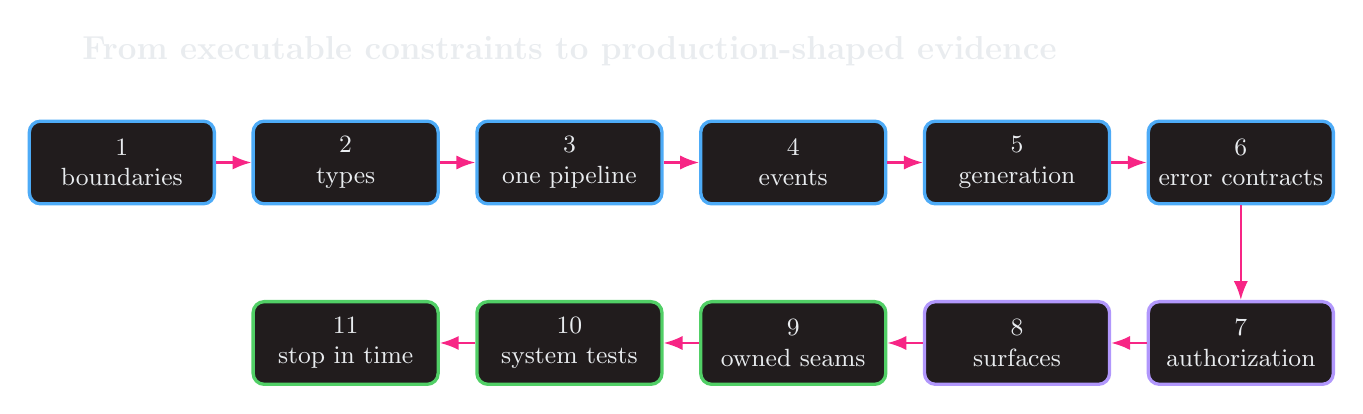
\begin{tikzpicture}[text=ink,lesson/.style={rounded corners=4pt,draw=blue,fill=panel,very thick,minimum width=2.35cm,minimum height=1.05cm,align=center,font=\small},arrow/.style={-{Latex[length=2.4mm]},thick,pink}]
 \node[lesson] (l1) {1\\boundaries}; \node[lesson,right=.45cm of l1] (l2) {2\\types};
 \node[lesson,right=.45cm of l2] (l3) {3\\one pipeline}; \node[lesson,right=.45cm of l3] (l4) {4\\events};
 \node[lesson,right=.45cm of l4] (l5) {5\\generation}; \node[lesson,right=.45cm of l5] (l6) {6\\error contracts};
 \node[lesson,draw=violet,below=1.2cm of l6] (l7) {7\\authorization};
 \node[lesson,draw=violet,left=.45cm of l7] (l8) {8\\surfaces};
 \node[lesson,draw=green,left=.45cm of l8] (l9) {9\\owned seams};
 \node[lesson,draw=green,left=.45cm of l9] (l10) {10\\system tests};
 \node[lesson,draw=green,left=.45cm of l10] (l11) {11\\stop in time};
 \draw[arrow] (l1)--(l2); \draw[arrow] (l2)--(l3); \draw[arrow] (l3)--(l4); \draw[arrow] (l4)--(l5); \draw[arrow] (l5)--(l6);
 \draw[arrow] (l6)--(l7); \draw[arrow] (l7)--(l8); \draw[arrow] (l8)--(l9); \draw[arrow] (l9)--(l10); \draw[arrow] (l10)--(l11);
 \node[font=\bfseries\large,text=ink,above=.55cm of l3] {From executable constraints to production-shaped evidence};
\end{tikzpicture}
\end{document}
